\documentclass[pdftex,12pt,a4paper]{report}
\usepackage[top=2cm, bottom=2.5cm, left=3cm, right=3cm]{geometry}
\usepackage[pdftex]{graphicx}
\usepackage{amsmath}
\usepackage{amsfonts}
\usepackage{listings}
\usepackage{subcaption}
\usepackage{capt-of}
\usepackage{amssymb}
\usepackage[utf8]{inputenc}
\usepackage{booktabs}
\usepackage{hyperref}
\usepackage{caption}
\newcommand{\HRule}{\rule{\linewidth}{0.5mm}}
\makeindex

\usepackage{todonotes}
\usepackage{amsmath}
\usepackage{float}
%\usepackage{subfigure}
\usepackage{braket}
%\usepackage[left=2.5cm,right=2.5cm,top=1.5cm,bottom=1cm,includeheadfoot]{geometry}

\usepackage{tikz}

%TikZ Package
%\usepackage{pgfplots}
%\usetikzlibrary{plotmarks}
%\usetikzlibrary{patterns}
%\usetikzlibrary{positioning}

%\usepgfplotslibrary{external} 
%\tikzexternalize
%\tikzsetexternalprefix{external_figs/}

\usepackage{textcomp}
\bibliographystyle{mybibstylemakebst}

\usepackage{wrapfig}
\usepackage{multicol}

\usepackage{lipsum}
\usepackage{scrextend}


\begin{document}
\begin{titlepage}
\begin{center}
Mathematisch-Naturwissenschaftlichen Fakultät I\\
Institut für Physik\\
Humboldt-Universität zu Berlin\\
\vspace{2cm}
\LARGE Computational Physics II\\
Final Project:\\
\LARGE Feedforward Neural Network
\vspace{2cm}
\end{center}
Submitted by:\\
Aron Ernesto Castro Martinez (566584)\\
Anna-Belle Garten (596556)\\
Max Pfeifer (567357)\\
Marius Pille (601844)
\\[1cm]

\noindent Advisor:\\
\hspace*{0.5cm} \textit{Dr. Agostino Patella}
\\[1cm]
%Deadline:\hspace*{0.5cm}  \textit{27.02.2019}
Submission: \hspace*{0.5cm}  \textit{27.02.2019}

\end{titlepage}

%\include{hyphenations}
\pagenumbering{Roman} 

\tableofcontents

%\listoffigures %Abbildungsverzeichnis

%\listoftables %Tabellenverzeichnis

%\chapter*{Abk"urzungsverzeichnis}
%\input{./Abkuerzungsverzeichnis.tex}
\newpage

\pagenumbering{arabic}
\chapter{Introduction}
In the 1950's \textit{Artificial Intelligence} (AI) was born as an academic discipline and, much like a see-saw, has since then experienced fluctuations in interest and optimism about its potential as an innovative technique to expand the paradigms in the technological field. \\
As computational power increased in the late 90's and early years of the 21st century, a new found attraction for creating \textit{intelligent} machines resurrected AI. This also bringing along teeming funding; research and development became a race and AI proved itself extremely useful in several different areas, such as computer science, economics, statistics, medicine, and robotics. The algorithms that are used to teach a machine how to \textit{think} and \textit{learn} from experience in order to achieve human-level performance at carrying out specific tasks are nowadays known as \textit{Machine Learning} (ML).\\
A new era had begun: data miners started analyzing the accessible, enormous amounts of information (\textit{Big Data}) with ML algorithms, to find patterns in a quest for actionable data, thus giving birth to a broader family of ML methods, denominated \textit{Deep Learning}. One particular breakthrough of Deep Learning was the invention of \textit{Artificial Neural Networks} (ANN). \\
The main concept behind an ANN is to deploy a framework, analogous to a biological neural network, that is able to unite many distinct ML algorithms to process complex data inputs and solve a specific problem at hand. ANNs have been successful in numerous assignments, including speech and image recognition. It is the latter that this project wishes to delve itself into - its core idea being to contrive and implement a \textit{Feedforward Neural Network} on MATLAB, to recognize handwritten numbers from the MNIST database. By no means is this an original approach; it is, notwithstanding, a good introductory way of attempting to comprehend the somewhat abstruse world of deep learning and Artificial Intelligence.
 

\chapter{Theoretical Concepts}
\section{Sigmoid Neurons}\label{sigNeuron}
The building blocks of every neural network are, evidently, the neurons. Each neuron is in charge of processing information, to do so it has individual weights for each input going into the neuron and a threshold for the activation of the neuron, the bias. The output, i.e. the activation value of the neuron, depends on how these two parameters were defined.\\
A very simple type of neuron is called a perceptron which uses a step function as the activation function for the neuron, that is, given a binary input it prompts a binary output as well; hence, networks of perceptrons can be used to compute any logical function. However, if the in-going information is not only 1's and 0's but the values lie somewhere in between the network will not process the information adequately. One way to obviate this issue is to choose a different activation function, the sigmoid function:
\begin{equation}
    \sigma(z) = \frac{1}{1 + exp(- \sum_j w_j x_j -b)}
\end{equation}

Where the $x_j$ are the inputs, $w_j$ their respective weights and $b$ the biases of each neuron; the quantity $z =\sum_j w_jx_j - b$ is called a weighted input. Due to the nature of the sigmoid function, a subtle alteration of the parameters causes only a small corresponding change in the output from the network, which allows the learning to be possible by carefully tailoring the weights and/or biases to match the network's output to the desired output.
 
\section{Designing a Neural Network}\label{designNN}

A neural network (NN) consists primordially of an input layer, an output layer and one or several intermediate layers called hidden layers.\\
The number of sigmoid neurons in the input layer is equal to the number of inputs in a sample of information, in the case of image recognition by sampling the MNIST database, there are 784 pixels in one image so the network needs 784 input neurons where each grayscale value for each pixel is stored. In the output layer there are, consequently, 10 neurons (one for each digit from 0 to 9). One essential aspect of designing a neural network is figuring out the appropriate number of hidden layers and the size - number of hidden neurons- of each layer. Please note that exaggerating about the size and number of hidden layers does not necessarily elicit a better trained network, all along greatly costing valuable computational resources.

\subsection*{Feedforward NN}\label{feedforwardNN}

 In a feedforward NN the output of a layer is the input of the next one, so the information is just fed in one direction: from the leftmost (input layer) to the rightmost layer (output layer); there are no loops allowed.

\section{Backpropagation}\label{backpTheo}

The Backpropagation algorithm is an algorithm that can be used to optimize the learning process of the network. It does so by finding out the values by which the weights and biases have to be changed, in order to achieve a higher accuracy of the network's goal. The main concepts used are: a cost function and its gradient.

\subsection{Cost Function}\label{costFuncTheo}

The cost function establishes quantitatively how well the network is classifying the inputs. For this network, the quadratic cost function (otherwise known as the mean squared error, MSE) was chosen:
\begin{equation}
    C(w,b) = \frac{1}{2 n} \sum^n_x \mid \mid y(x) - a \mid \mid ^2
\end{equation}
Where $w,b$ denote the weights and biases respectively, $n$ is the total number of training inputs, $a$ is the vector of output values (activation values) for each input $x$. Minimizing the cost as a function of the weights and biases is the main idea behind a training algorithm, like backpropagation.

\subsection{Gradient Descent}\label{gradDescTheo}

When discussing minimization problems, the gradient descent algorithm proposes a nice and effective way to solve them. In this particular case, the algorithm will determine the set of these two parameters which minimize the cost function.\\
The idea is to compute the gradient of the cost function -to see the influence of each weight and bias- and then adjust the weights and biases accordingly, that is, decrease their value by a small positive amount so that they "move" down the slope of the cost function until they reach a global minimum. To be laconic, gradient descent is a method where each new step is taken in the direction which does most to immediately decrease the cost function. This is another reason why the MSE function was selected as the cost function, because it is a smooth well-behaved function that allows to easily find the best adjustment over the weights and biases for the improvement of the network. The euqations are defined as
\begin{equation}
    w \rightarrow w' = w -\eta \frac{\partial C }{\partial w} 
\end{equation}
\begin{equation}
    b \rightarrow b' = b -\eta \frac{\partial C }{\partial b} 
\end{equation}

With $\nabla = (\frac{\partial C }{\partial w}  , \frac{\partial C }{\partial b} )$ the gradient of the cost function; $w$, $w'$, $b$ and $b'$ the old and new weights and biases respectively; and $\eta$ the learning rate, which should be a small positive integer. 

\subsection{Stochastic Gradient Descent}\label{SGDtheo}

In a large network calculating the gradient of the cost function for each weight and bias implies a proportionally large computational cost. A good segue to avert this situation, is to use an algorithm called stochastic gradient descent (SGD) to expedite the computation. The idea is to divide an entire data-set into batches and estimate the gradient for each one of them. Averaging over the number of batches, the value of the gradient per batch is roughly equal to the gradient of the whole data-set, provided the size of each batch is large enough. In this way, the learning process is speed up, while obtaining a good estimate of the true gradient.  


\chapter{Implementation}
In this section, a program to train a feedforward neural network with one hidden layer is described using pseudocode. It learns how to recognize handwritten digits from the MNIST database applying a stochastic gradient descent algorithm. Before starting with the rundown through the code, it is necessary a few key points are described pertaining  .

\section{Data structure}\label{DataStruct}
 The diagram below provides an overview of the main program divided in sections, to facilitate a quick and general understanding of the purpose of the functions and algorithms used in the project.\\
 
%begin{comment}
%:Title: Work breakdown structures aka WBS diagrams
%:Tags: Charts;Diagrams;Trees
%:Author: Gonzalo Medina
%:Slug: work-breakdown-structure

%A work breakdown structure (WBS) diagram, is for decomposing a task into smaller parts, which helps organizing and performing. This example diagram shows possible tasks for designing a TikZ diagram. The basis is a tree, nodes were addes below its child nodes. It was originally posted by Gonzalo Medina as TeX.SE (http://tex.stackexchange.com/q/81809/213), modified by Stefan Kottwitz.
%\end{comment}
\usetikzlibrary{arrows,shapes,positioning,shadows,trees}

\tikzset{
  basic/.style  = {draw, text width=3cm, drop shadow, font=\sffamily, rectangle},
  root/.style   = {basic, rounded corners=2pt, thin, align=center,
                   fill=blue!30},
  level 2/.style = {basic, rounded corners=6pt, thin,align=center, fill=gray!30,
                   text width=8em},
  level 3/.style = {basic, thin, align=left, fill=brown!60, text width=6.5em, scale = 0.9}
}

\begin{tikzpicture}[
  level 1/.style={sibling distance=40mm},
  edge from parent/.style={->,draw},
  >=latex,
  scale= 0.9
  ,every node/.style={scale= 0.9}]

% root of the the initial tree, level 1
\node[root] {inputControl}
% The first level, as children of the initial tree
  child {node[level 2] (c1) {loadMNISTImages \& Labels}}
  child {node[level 2] (c2) {ffNetwork}}
  child {node[level 2] (c3) {trainNetwork}}
  child {node[level 2] (c4) {testNetwork}};

% The second level, relatively positioned nodes
\begin{scope}[every node/.style={level 3}]
\node [below of = c1, xshift=15pt, yshift = - 7pt] (c11) {Load the MNIST data};

\node [below of = c2, xshift=15pt] (c21) {Define the parameters};
\node [below of = c21, yshift = -3.5pt] (c22) {build the structure};

\node [below of = c3, xshift=15pt] (c31) {train the network};
\node [below of = c31, yshift = -12pt] (c32) {Execute the backpropagation algorithm};
\node [below of = c32, yshift = -19pt] (c33) {Calculate the gradient descent};
\node [below of = c33, yshift = -11pt] (c34) {Determine the cost function};


\node [below of = c4, xshift=15pt] (c41) {Test the trained network};

\end{scope}

% lines from each level 1 node to every one of its "children"
\foreach \value in {1}
  \draw[->] (c1.195) |- (c1\value.west);

\foreach \value in {1,2}
  \draw[->] (c2.195) |- (c2\value.west);

\foreach \value in {1,2,3,4}
  \draw[->] (c3.195) |- (c3\value.west);
  
\foreach \value in {1}
  \draw[->] (c4.195) |- (c4\value.west);
  
  
  
\end{tikzpicture}\\
 
 In \textit{inputControl} you can set the parameters i.e. the number of minibatches, the number of neurons of each layer and the number of hidden layers. Included are four main functions \textit{loadMNISTImages}, \textit{Labels}, \textit{ffNetwork}, \textit{ trainNetwork} and the \textit{testNetwork}. The diagram describes the content of the functions. The structure of the program is clear and straight forward.\\
 
 Another important aspect when writing the code to train a network, is to decide how the data is going to be managed and stored. Generally, the programming language has some influence on the decision, due to the fact that different programs work on distinct programming bases. It is good practice to use matrices when programming in MATLAB, nevertheless, in our case we use cell arrays to store the weights and biases of the system, due to a versatile feature they possess: information can be stored in cell arrays regardless of data type and size. These can afterwards be listed in a structure array for clarity's sake. Using structures enables us to store any type of data in containers called fields, that way all the information can be grouped in one single variable, while allowing an easy access to single small groups of information. However, a few issues remain, for instance, cell arrays require more processing time than matrices.\\
 Considering the problem in question and given the relative simplicity of our neural network, we reached a compromise between an organized easy-to-follow structure over fast computing. Therefore, the numerical data for each layer is stored in cell arrays and these, in a structure array, e.g.:
 
 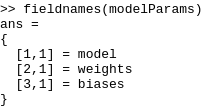
\includegraphics[scale=0.8]{Bilder/structArray.png}
 
 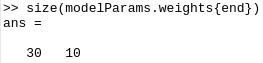
\includegraphics[scale=0.8]{Bilder/weightsMat.png}

\section{Algorithms}\label{Algorithms}

In this section we will present the main algorithms used to train the neural network as well as to test its performance and functioning. The description follows in pseudocode form.\\
\rule{\textwidth}{0.4pt}
 FEEDFORWARD: Returns the cell arrays "unactivatedOutput" and "activatedOutput" with the weighted inputs and activation values for each layer of the network after applying the feedforward algorithm iteratively. Returns a 1 if the input was correctly classified or a 0 if incorrectly in "classifiedCorrect".\\
\rule{\textwidth}{0.4pt}
\begin{addmargin}[2em]{0em}
\textbf{function} evaluate( \textbf{struct} modelParams, \textbf{double} data, dataLabel )\\
    $- \qquad$ \textbf{local variables:} int x[length(modelParams.model.hidden)]\\
    $- \qquad$ activatedOutput$_{input}$ $\leftarrow$ data\\
    $- \qquad $\\
    $- \quad $ \textit{Forward feeding}\\
    $- \qquad $ \textbf{for all} k = 2,3,...,x-1 \textbf{do}\\
    $- \qquad \quad $ unactivatedOutput $_k$ 
    $\leftarrow$ activatedOutput $_{k}*$ weights$_{k}$ - biases$_{k}$ \\
    $- \qquad \quad $ activatedOutput $_{k+1}$ 
    $\leftarrow$ activate(unactivatedOutput $_k$)\\
    $- \qquad $ \textbf{end for}\\
    $- \qquad $\\
    $- \quad $ \textit{Control}\\
    $- \qquad $ \textbf{if} activatedOutput $_{output}$ $\Longleftrightarrow$ dataLabel\\
    $- \qquad \quad$ classifiedCorrect $\leftarrow$ 1\\
    $- \qquad$ \textbf{end if}\\
    $- \qquad$ \textbf{return} classifiedCorrect, activatedOutput,  unactivatedOutput\\
\textbf{end function}\\
\end{addmargin}
\rule{\textwidth}{0.4pt}
 BACKPROPAGATION: Returns the cell arrays "deltaGradWeights" and "deltaGradBiases" with the gradient of the cost function for the weights and the biases respectively calculated with the backpropagation algorithm.\\
\rule{\textwidth}{0.4pt}
\begin{addmargin}[2em]{0em}
\textbf{function} backprop( \textbf{struct} modelParams, \textbf{double} data, dataLabel )\\
    $- \qquad$ \textbf{local variables:} int x[length(modelParams.model.hidden)+2]\\
    $- \qquad$ unactivatedOutput, activatedOutput $\leftarrow$ evaluate(modelParams, data)\\
    $- \qquad $\\
    $- \quad $ \textit{Propagating the gradient bacwards starting at output layer}\\
    $- \qquad$ deltaGradBiases$_{output}$ $\leftarrow$ deriveCost(dataLabel, activatedOutput${_x}$)\\
    $- \qquad$ deltaGradWeights$_{output}$ $\leftarrow$ activatedOutput$_{x-1}*$ deltaGradBiases$_{output}$\\
    $- \qquad $ \textbf{for all} k = 2,3,...,x-1 \textbf{do}\\
    $- \qquad \quad $ deltaGradBiases $_{x-k}$ 
    $\leftarrow$ deltaGradBiases$_{x-k+1}*$modelParams.weights$_{x-k+1}$\\
    $- \qquad \quad $ deltaGradWeights $_{x-k}$ 
    $\leftarrow$ activatedOutput$_{x-k}*$ deltaGradBiases$_{x-k}$\\
    $- \qquad $ \textbf{end for}\\
    $- \qquad$ \textbf{return} deltaGradWeights, deltaGradBiases\\
\textbf{end function}\\
\end{addmargin}
\rule{\textwidth}{0.4pt}
 ADJUSTING PARAMETERS: Returns the updated structure array "modelParams" after applying the backpropagation algorithm on each input of a single batch.\\
\rule{\textwidth}{0.4pt}
\begin{addmargin}[2em]{0em}
\textbf{function} adjustParams( \textbf{struct} modelParams, \textbf{double} data, dataLabel )\\
    $- \qquad$ \textbf{local variables:} int x[length(data)]\\
    $- \qquad $ \textbf{for all} k = 1,2,...,x \textbf{do}\\
    $- \qquad \quad$ deltaGradWeights, deltaGradBiases $\leftarrow$\\
    $- \qquad \qquad \quad \qquad $ backprop(modelParams, data$_{k}$  , dataLabel$_{k}$)\\
    $- \qquad $\\
    $- \qquad $ \textit{Updating weights and biases}\\
    $- \qquad \quad$ \textbf{local variables:} int y[length(deltaGradWeights)]\\
    $- \qquad \quad $ \textbf{for all} l = 1,2,...,y \textbf{do}\\
    $- \qquad \quad \quad$ modelParams.weights$_{l}$ $\leftarrow$ modelParams.weights$_{l}$ - eta/x $*$deltaGradWeights$_{l}$\\
    $- \qquad \quad \quad$ modelParams.biases$_{l}$ $\leftarrow$ modelParams.biases$_{l}$ - eta/x $*$deltaGradBiases$_{l}$\\
    $- \qquad \quad$ \textbf{end for}\\
    $- \qquad$ \textbf{end for}\\
    $- \qquad$ \textbf{return} modelParams\\
\textbf{end function}\\
\end{addmargin}
\rule{\textwidth}{0.4pt}
 TRAINING: Returns the structure array "modelParams" with the network's final parameters after training it using stochastic gradient descent with two stopping criteria: "accuracy" and maximum number of iterations. Returns the vector "cost" with the value of the cost function after every iteration and the value "epoch" with the total number of iterations.\\
\rule{\textwidth}{0.4pt}
\begin{addmargin}[2em]{0em}
\textbf{function} trainNetwork( \textbf{struct} model, \textbf{double} data, dataLabel )\\
    $- \qquad$ \textbf{local variables:} int epoch, x[length(data(:,1))], y[batchSize]\\
    $- \qquad $ \textbf{while} model.averageCostChange $>$ accuracy \textbf{AND} epoch$<$100 \textbf{do}\\
    $- \qquad \quad$ epoch $\leftarrow$ epoch + 1\\
    $- \qquad $\\
    $- \qquad $ \textit{Learning}\\
    $- \qquad \quad$ \textbf{for all} k = 1,2,...,x/y \textbf{do}\\
    $- \qquad \quad \quad  $ modelParams $\leftarrow$ adjustParams(modelParams,data$_k$, dataLabel$_k$) \\ 
    $- \qquad \quad $ \textbf{end for}\\
    $- \qquad $\\
    $- \qquad $ \textit{Calculating cost of an iteration}\\
    $- \qquad \quad $ cost $_{epoch}$
    $\leftarrow$ calcCost(modelParams, data, dataLabel)\\
    $- \qquad \quad$ \textbf{if} mod(epoch, model.averageOverEpochs) == 0\\
    $- \qquad \quad \quad$ \textbf{for all} k = 1,2,...,model.averageOverEpochs - 1 \textbf{do}\\
    $- \qquad \quad \quad \quad $costChange $\leftarrow$ cost$_{epoch-k+1}$ - cost$_{epoch-k}$\\
    $- \qquad \quad \quad$ \textbf{end for}\\
    $- \qquad \quad$ model.averageCostChange $\leftarrow$\\
    $- \qquad \quad \quad \quad \quad$ abs(sum(costChange)/(model.averageOverEpochs - 1))\\
    $- \qquad \quad$ \textbf{end if}\\
    $- \qquad$ \textbf{end while}\\
    $- \qquad$ \textbf{return} modelParams, cost, epoch\\
\textbf{end function}\\
\end{addmargin}
\rule{\textwidth}{0.4pt}
 TESTING: Returns the value of the ratio of correctly identified inputs over total number of inputs.\\
\rule{\textwidth}{0.4pt}
\begin{addmargin}[2em]{0em}
\textbf{function} testNetwork( \textbf{struct} modelParams, \textbf{double} data, dataLabel )\\
    $- \qquad$ \textbf{local variables:} int x[length(data(:,1))]\\
    $- \qquad $\\
    $- \quad $ \textit{Forward feeding to get output on test-set with trained network}\\
    $- \qquad $ \textbf{for all} k = 1,2,...,x \textbf{do}\\
    $- \qquad \quad $ results$_k$ $\leftarrow$ evaluate( modelParams,  data$_{k}$, dataLabel$_{k}$)\\
    $- \qquad $ \textbf{end for}\\
    $- \qquad $\\
    $- \quad $ \textit{Computing accuracy}\\
    $- \qquad $ modelResult $\leftarrow$ sum(results)/(length(results))\\
    $- \qquad$ \textbf{return} modelResult\\
\textbf{end function}\\
\end{addmargin}

The pseudocode below shows the way to run the code and get the sought-after information:\\
\rule{\textwidth}{0.4pt}
\textbf{inputControl:} TRAINING AND TESTING A FF-NEURAL NETWORK\\
\rule{\textwidth}{0.4pt}
\rule{\textwidth}{0.4pt}
NETWORK'S CHARACTERISTICS AND HYPER-PARAMETERS: Defining the learning rate "eta", the size of the batches in which the data-set is divided for the SGD "batchSize", and the activation function and its derivative in the object "activationFunction" of the class "activation".\\
\rule{\textwidth}{0.4pt}
\rule{\textwidth}{0.4pt}
\begin{addmargin}[2em]{0em}
\textbf{global variables:} \\
$- \qquad$ \textbf{double} eta\\
$- \qquad$ \textbf{double} batchSize\\
$- \qquad$ \textbf{activation} activationFunction (@sig, @sigDerivative)\\
$-$\\
\textbf{Loading MNIST data}\\
$- \qquad$ testData $\leftarrow$ loadMNISTImages('path to testing images')\\
$- \qquad$ testLabel $\leftarrow$ loadMNISTLabels('path to testing images' labels')\\
$- \qquad$ trainData $\leftarrow$ loadMNISTImages('path to training images')\\
$- \qquad$ trainLabel $\leftarrow$ loadMNISTLabels('path to training images' labels')\\
$-$\\
\textbf{Network's configuration}\\
$- \qquad$ model $\leftarrow$ ffNetwork(activationFunction, eta, batchSize, 784, 10, 30)\\
$-$\\
\textbf{Procedure:} TRAINING\\
$- \qquad$ modelParams, cost, epoch $\leftarrow$ trainNetwork(model, trainData, \\
$- \qquad \qquad  $trainLabel)\\
$-$\\
\textbf{Procedure:} TESTING\\
$- \qquad$ modelResult $\leftarrow$ testNetwork(modelParams, testData, testLabel)\\
\end{addmargin}

\section{Functions}\label{Functions}

In this section each of the functions utilized by the training and testing algorithms are listed.\\
\rule{\textwidth}{0.4pt}
PARSING DATA: Returns matrix "images" of size (number of images X 784 pixels) with the images and column vector "labels" of size (number of labels X 1) with the labels for each image from the MNIST data-set.\\
\rule{\textwidth}{0.4pt}
\begin{addmargin}[2em]{0em}
\textbf{function} loadMNISTImages(\textbf{string} path to images)\\
    $- \qquad$fp $\leftarrow$ open path to images\\
    $- \qquad$images $\leftarrow$ read fp\\
    $- \qquad$ \textbf{return} images\\
\textbf{end function}\\
\end{addmargin}
\begin{addmargin}[2em]{0em}
\textbf{function} loadMNISTLabels(\textbf{string} path to labels)\\
$- \qquad$ fp $\leftarrow$ open path to labels\\
    $- \qquad$ labels $\leftarrow$ read fp\\
    $- \qquad$ \textbf{return} labels\\
\textbf{end function}\\
\end{addmargin}
\rule{\textwidth}{0.4pt}
ACTIVATION: Defines a class "activation". The objects from this class have the methods "activate" and "deriveActivation" which computes the activation function on an input and its derivative respectively.\\
\rule{\textwidth}{0.4pt}
\begin{addmargin}[2em]{0em}
\textbf{class} activation\\
    $- \qquad$\textbf{properties}\\
    $- \qquad \quad$ activate\\
    $- \qquad \quad$ deriveActivation\\
    $- \qquad$ \textbf{end properties}\\
    $- \qquad$ \textbf{methods}\\
    $- \qquad \quad$ \textbf{function} activation(Function, Derivative)\\
    $- \qquad \quad \quad $obj.activate $\leftarrow$ Function\\
    $- \qquad \quad \quad $obj.deriveActivation $\leftarrow$ Derivative\\
    $- \qquad \quad$ \textbf{end function}\\
    $- \qquad$ \textbf{end methods}\\
\textbf{end class}\\
\end{addmargin}
\rule{\textwidth}{0.4pt}
SIGMOID FUNCTION: Returns the vector "result" with the calculated sigmoid function of an input "x".\\
\rule{\textwidth}{0.4pt}
\begin{addmargin}[2em]{0em}
\textbf{function} sig( \textbf{double} x )\\
    $- \qquad$ result $\leftarrow$ sigmoid function x \\
    $- \qquad$ \textbf{return} result\\
\textbf{end function}\\
\end{addmargin}
\rule{\textwidth}{0.4pt}
DERIVATIVE SIGMOID FUNCTION: Returns the vector "result" with the calculated derivative of a sigmoid function of an input "x".\\
\rule{\textwidth}{0.4pt}
\begin{addmargin}[2em]{0em}
\textbf{function} sigDerivativ( \textbf{double} x )\\
    $- \qquad$ result $\leftarrow$ sigmoid function derivative x \\
    $- \qquad$ \textbf{return} result\\
\textbf{end function}\\
\end{addmargin}
\rule{\textwidth}{0.4pt}
DERIVATIVECOST FUNCTION: Returns the vector "dC" with the calculated derivative of the cost function of an input "actualOutput" and the desired value to the input "desiredOutput".\\
\rule{\textwidth}{0.4pt}
\begin{addmargin}[2em]{0em}
\textbf{function} deriveCost( \textbf{double} desiredOutput, actualOutput)\\
    $- \qquad$ dC $\leftarrow$ actualOutput - desiredOutput \\
    $- \qquad$ \textbf{return} desiredOutput, actualOutput\\
\textbf{end function}\\
\end{addmargin}
\rule{\textwidth}{0.4pt}
CONFIGURING NETWORK: Returns the structure array "model" loaded with all necessary parameters to create the initial network.\\
\rule{\textwidth}{0.4pt}
\begin{addmargin}[2em]{0em}
\textbf{function} ffNetwork( \textbf{activation} af, \textbf{double} eta, batchsize, in, hid, out )\\
    $- \qquad$ model $\leftarrow$ af, eta, batchsize, in, hid, out \\
    $- \qquad$ \textbf{return} model\\
\textbf{end function}\\
\end{addmargin}
\rule{\textwidth}{0.4pt}
INITIALIZING NETWORK: Returns the cell arrays "weights" and "biases" with the randomly generated weights and biases for each layer of the initial network.\\
\rule{\textwidth}{0.4pt}
\begin{addmargin}[2em]{0em}
\textbf{function} ffNetwork( \textbf{struct} model )\\
    $- \qquad$ \textbf{local variables:} int x[length(model.hidden)]\\
    $- \qquad$ weights$_{input}$, biases$_{input}$ $\leftarrow$ randn(model.input)\\
    $- \qquad$ \textbf{if} x $>$ 1\\
    $- \qquad \quad $ \textbf{for all} k = 2,3,...,x \textbf{do}\\
    $- \qquad \qquad \quad $ weights$_k$ $\leftarrow$ randn(model.hidden(k-1),model.hidden(k))\\
    $- \qquad \qquad \quad $ biases$_k$$\leftarrow$ randn(model.hidden(k))\\
    $- \qquad \quad $ \textbf{end for}\\
    $- \qquad $ \textbf{end if}\\
    $- \qquad$ weights$_{output}$, biases$_{output}$ $\leftarrow$ randn(model.output)\\
    $- \qquad$ \textbf{return} weights, biases\\
\textbf{end function}\\
\end{addmargin}
\rule{\textwidth}{0.4pt}
 CALCULATE COST: Returns the value of the cost function for a set of inputs "data" and corresponding expected outputs "labels".\\
\rule{\textwidth}{0.4pt}
\begin{addmargin}[2em]{0em}
\textbf{function} calcCost( \textbf{struct} modelParams, \textbf{double} data, dataLabel )\\
    $- \qquad$ \textbf{local variables:} int x[size(data,1)], double costVec, labelsVec\\
    $- \qquad $ \textbf{for all} k = 2,3,...,x \textbf{do}\\
    $- \qquad \quad $ labelsVec(dataLabel$_k$ + 1)$\leftarrow$ 1 \\ 
    $- \qquad \quad $ activatedOutput $\leftarrow$ evaluate( modelParams,  data$_{k}$, dataLabel$_{k}$)\\
    $- \qquad \quad $ costVec $_{k}$
    $\leftarrow$ norm(labelsVec - activatedOutput)$^2$\\
    $- \qquad \quad $ labelsVec(dataLabel$_k$ + 1)$\leftarrow$ 0 \\ 
    $- \qquad $ \textbf{end for}\\
    $- \qquad $ cost $\leftarrow$ sum(costVec)/(2 $*$ x)\\
    $- \qquad$ \textbf{return} cost\\
\textbf{end function}\\
\end{addmargin}

\section{Testing}
\subsection{Test: decrease of cost function}
To test our implementation, specifically to verify that the learning works as expected, we evaluated the cost function along the training process and checked if it actually decreased. Figure \ref{fig:costTrainSet} shows two cost curves for the same parameter bundle (detailed parameters in the image caption) but different learning rates evaluated on the training set. In both cases it can be clearly seen that the cost is decreasing after each epoch and thereafter saturates at a level close to zero. While for a learning rate of eta = 3 the cost curve has some bumps in it and even slightly increases from epoch 12 to 13, the cost curve with eta = 0.5 is much smoother but also takes more than twice as many epochs to reach a comparable cost level. 
\begin{figure}[t!]
\centering
    \begin{subfigure}[t]{0.49\textwidth}
        \centering
        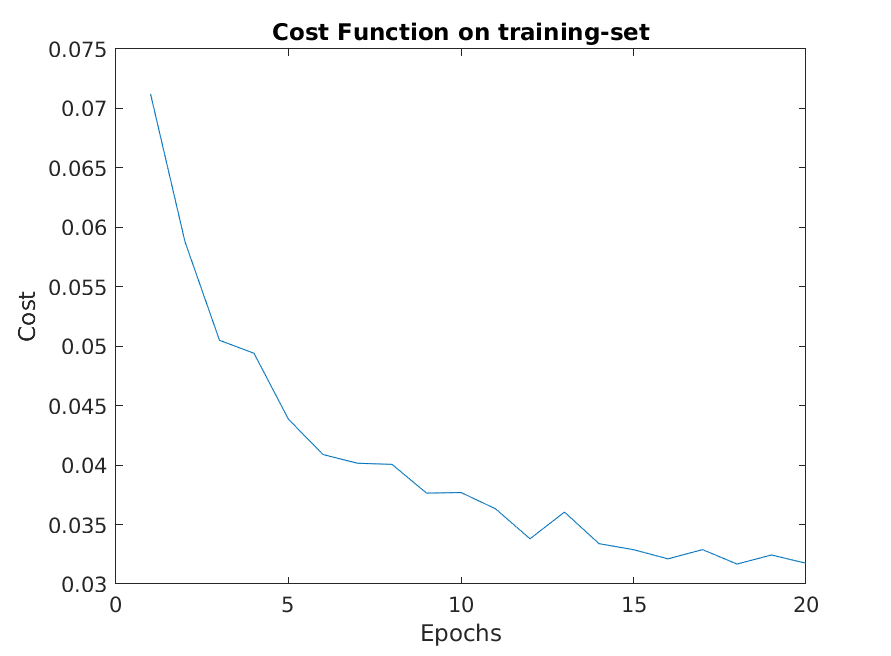
\includegraphics[width=1.1\textwidth]{test_src/img/eta3_trainset}
        \caption{learning rate eta = 3.0}
    \end{subfigure}
    \begin{subfigure}[t]{0.49\textwidth}
        \centering
        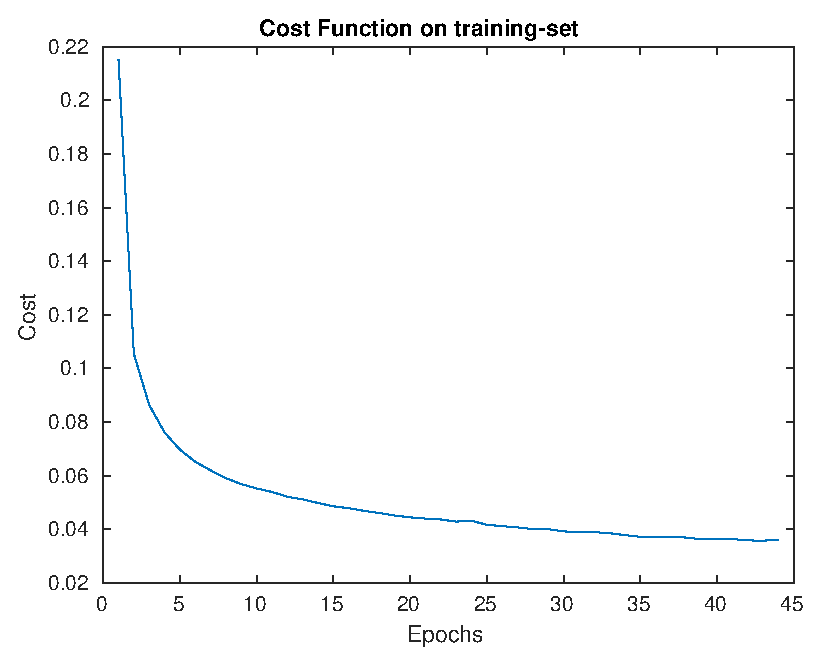
\includegraphics[width=1.1\textwidth]{test_src/img/eta05_trainset}
        \caption{learning rate eta = 0.5}
    \end{subfigure}
    \caption{Cost function evaluated on the whole training set (60000 inputs) with a batch size of 10 and 30 neurons in the hidden layer. }
    \label{fig:costTrainSet}
\end{figure}

% (in the following referred as epoch curve)

\subsection{Test: the backpropagation algorithm}
The backpropagation algorithm in the \textit{backprop.m} file is used to calculate the gradient of the cost function in respect to all weights and biases. To check if the algorithm is implemented correctly, the same derivatives can be calculated in a numerical way using equation \eqref{eq:numDerivativ}, where $v$ is a random number and $\epsilon$ goes to zero.
\begin{align}
    f'(x) = \lim_{\epsilon \to 0} \frac{f(x + \epsilon \times v) - f(x - \epsilon \times v )}{2\epsilon}
    \label{eq:numDerivativ}
\end{align}
According to the equation above the difference of the numeric and the analytic derivatives $g(x)$ should approach zero as $\epsilon$ gets smaller. That is:
\begin{align}
f'(x) -v\times g(x) = \mathcal{O}(\epsilon)
    \label{eq:condition}
\end{align}
The matlab script \textit{backpropTest.m} uses equation \eqref{eq:condition} to ascertain the right implementation of the backpropagation algorithm. It uses an empirical value for the learning rate $\epsilon$ of $10^{-4}$ \footnote{\url{http://ufldl.stanford.edu/wiki/index.php/Gradient_checking_and_advanced_optimization}}, and corroborates condition \eqref{eq:condition} for each weight and bias of a network. It has shown that the difference is of the magnitude $\mathcal{O}(10^{-12})$, for all weights and biases, which can be taken as a proof that the backpropagation algorithm is correct.  

\chapter{Results \& Discussion}

\section{Influence of hyperparameters}\label{params}

In order to investigate how the network's learning behavior depends on the size of the training set and other hyperparameters, such as the learning rate, batch size and number of neurons in the hidden layer, we used the \textit{costOverEpochs()} function and the script \textit{costDiffParams()}.
The \textit{costOverEpochs()} function is very similar to the \textit{trainNetwork()} function. It trains a neural network with one hidden layer and a given set of network parameters for
a fixed number of epochs. Thereafter it evaluates the cost function after each epoch on the test dataset and returns the epoch-evolution of the cost function. The script \textit{costDiffParams} is then used to generate cost vs. epoch curves for different parameter bundles. In the course of this, only one network parameter is changed at a time while the others (variables with the suffix 'Usual' in the script) are kept constant.

Figure \ref{fig:costTestset_sizeTrain} shows the cost curves for different numbers of training inputs (details in the plot). One recognizes that for a larger training set the cost decreases more faster and saturates at a lower absolute cost value, which meets our expectations.

Figure \ref{fig:costTestset_eta} shows the cost curves for different learning rates, whereby the whole training set was used to train the network. For a small learning rate of 0.6 the cost decreases more slowly compared to larger learning rates and is comparably smooth, but also saturates at a higher absolute cost value. Whereas the curve remains smooth for a learning rate of 1.0, it gets bumpy for larger learning rates which is likely due to overshooting (the learning rate is so high, that it overshoots the optimal point).

Figure \ref{fig:costTestset_batchSize} depicts the cost curves for different batch sizes. For a very small batch size of just 2 training inputs, the cost rapidly decreased after the first epoch but exhibits the most bumpy behaviour. This is probably due to individual training inputs being too much weighted during the adjustment of the network parameters, which results in the temporary optimization of the weights and biases just on these inputs. For a (comparably large) batch size of 250 training inputs, the cost decreases more slowly than with smaller batches. It also doesn't seem to be saturated after 20 epochs. The degregation of gradient descent based feedforward neural networks trained with a large batch size is a common issue and the reason is still investigated\footnote{N. S. Keskar, \textit{et al.}, \textit{On Large-Batch Training for Deep Learning: Generalization Gap and Sharp Minima}, ICLR (\textbf{2017})}.

Figure \ref{fig:costTestset_numNeurons} shows the cost curves for a varying number of neurons in the hidden layer. NEW PLOT

\newpage
\begin{figure}[h!]
\centering
    \centering
    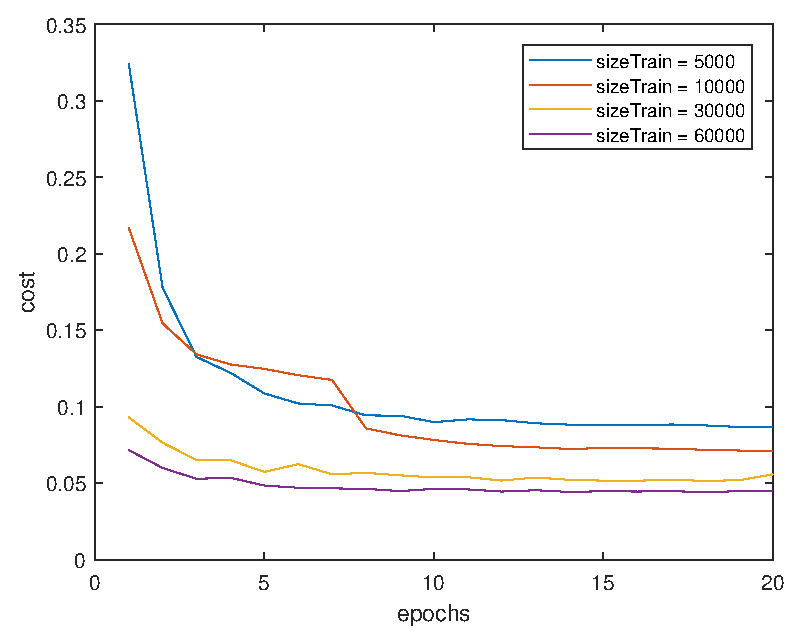
\includegraphics[width=0.92\textwidth]{test_src/img/20epochs/costOverEpochs_sizeTrain}
    \caption{Cost over 20 epochs for different sizes of the training set, a learning rate of 3, a batch size of 10 and 30 neurons in the hidden layer}
    \label{fig:costTestset_sizeTrain}
\end{figure}
\begin{figure}[h!]
\centering
    \centering
    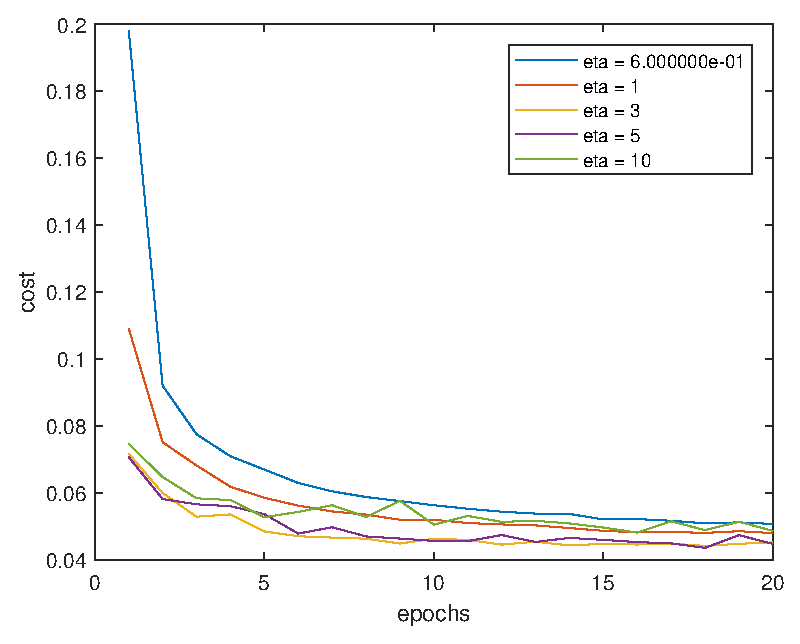
\includegraphics[width=0.92\textwidth]{test_src/img/20epochs/costOverEpochs_eta}
    \caption{Cost over 20 epochs for different learning rates, the whole training set (60000 inputs), a batch size of 10 and 30 neurons in the hidden layer}
    \label{fig:costTestset_eta}
\end{figure}

\newpage
\begin{figure}[h!]
\centering
    \centering
    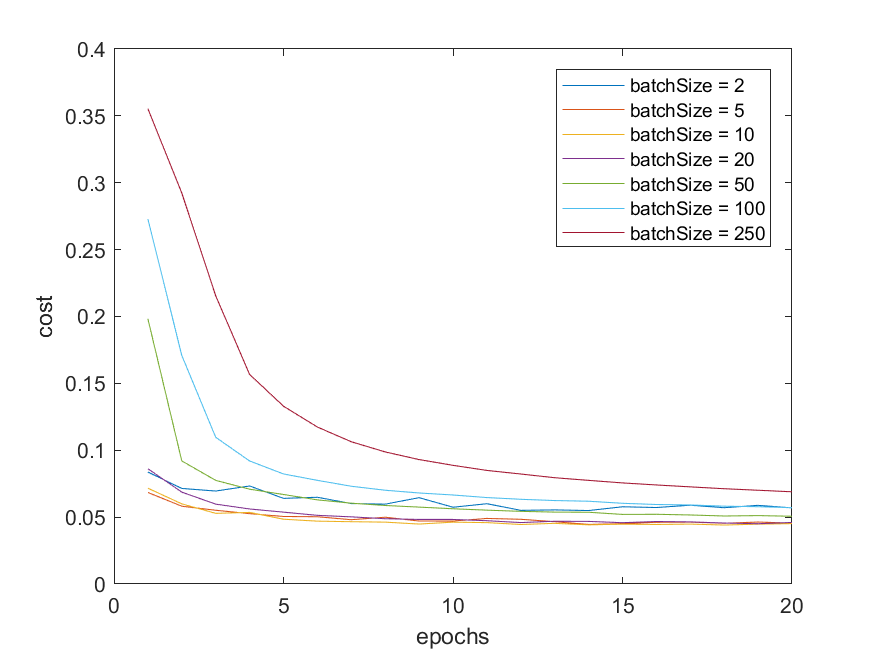
\includegraphics[width=0.91\textwidth]{test_src/img/20epochs/costOverEpochs_batchSize}
    \caption{Cost over 20 epochs for different batch sizes, the whole training set (60000 inputs), a learning rate of 3 and 30 neurons in the hidden layer}
    \label{fig:costTestset_batchSize}
\end{figure}
\begin{figure}[h!]
\centering
    \centering
    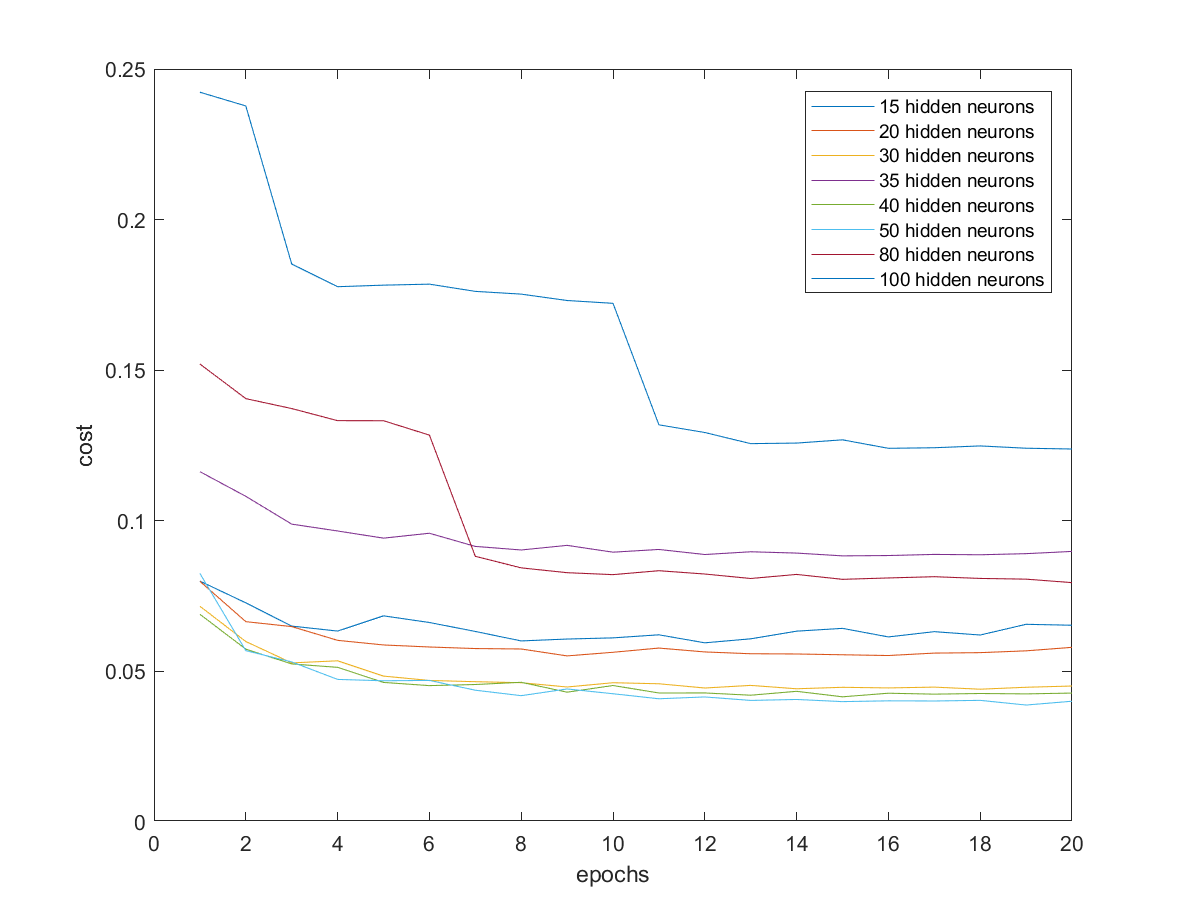
\includegraphics[width=0.91\textwidth]{test_src/img/20epochs/costOverEpochs_numNeurons}
    \caption{Cost over 20 epochs for numbers of neurons in the hidden layer, the whole training set (60000 inputs) and a batch size of 10}
    \label{fig:costTestset_numNeurons}
\end{figure}

%In addition for the number of neurons, the computation time needed to train the network and evaluate the cost function is plotted.

\section{Performance on MNIST Database}\label{detRate}


\chapter{Summary}
During this project we gained a lot of insights and knowledge on how neural networks work and what is possible and impossible with machine learning.
But we also learned a lot on a more general level, like how to improve your code by testing and working as a team on a software project. This chapter is a summary of these findings and it gives a short outlook on how this project could be improved in the future.  
\section{Lesson learned}
\textbf{Define a common base:} In the beginning everyone wrote their own version of what we thought was a neural network. This made it hard to compare our code because everyone structured it differently and used other cryptic names for the variables and functions. After we agreed on a common set of necessary function and a way to name variables it got much easier to understand the code of another and work as a team. \\
\textbf{Review the code:} Sometimes you get blind for your own code. You spent hours on finding a, in the end trivial, mistake. A fresh view can speed up this process and therefore it saved us a lot of time asking team mates for a code review.  \\
\textbf{Test your code helps to find and prevent bugs:} Testing forces you to cut your program in as small as possible functions,  which by itself already decreases bugs because these functions are easier to understand and you think more about the structure of your program. Also these tests verify certain functions and speed up the error search for new bugs.

\section{What next?}
In the course of this project we only implemented a simple version of a feedforward neural network with stochastic gradient descent with plenty of room for optimization. One way to improve our program would be to learn more about how matlab works and then speed up the calculations, decreasing the time needed for our network to train preparing it for more advanced data sets.  There are also many ways to tweak the stochastic gradient descent algorithm for faster learning and preventing it from getting stuck in local minima, that we put  aside in the limited time of the project but otherwise would be quite interesting. 


\end{document}